\documentclass[letterpaper,compsoc,twoside,onecolumn]{IEEEtran}
% generated by Docutils <https://docutils.sourceforge.io/>
\usepackage{cmap} % fix search and cut-and-paste in Acrobat
\usepackage{ifthen}
\usepackage[T1]{fontenc}
\usepackage{amsmath}
\usepackage{color}

\usepackage[font={small,it},labelfont=bf]{caption}
\usepackage{float}

\setcounter{secnumdepth}{0}

%%% Custom LaTeX preamble
\usepackage{scipy}
\makeatletter
\def\PY@reset{\let\PY@it=\relax \let\PY@bf=\relax%
    \let\PY@ul=\relax \let\PY@tc=\relax%
    \let\PY@bc=\relax \let\PY@ff=\relax}
\def\PY@tok#1{\csname PY@tok@#1\endcsname}
\def\PY@toks#1+{\ifx\relax#1\empty\else%
    \PY@tok{#1}\expandafter\PY@toks\fi}
\def\PY@do#1{\PY@bc{\PY@tc{\PY@ul{%
    \PY@it{\PY@bf{\PY@ff{#1}}}}}}}
\def\PY#1#2{\PY@reset\PY@toks#1+\relax+\PY@do{#2}}

\@namedef{PY@tok@w}{\def\PY@tc##1{\textcolor[rgb]{0.73,0.73,0.73}{##1}}}
\@namedef{PY@tok@c}{\let\PY@it=\textit\def\PY@tc##1{\textcolor[rgb]{0.25,0.50,0.56}{##1}}}
\@namedef{PY@tok@cp}{\def\PY@tc##1{\textcolor[rgb]{0.00,0.44,0.13}{##1}}}
\@namedef{PY@tok@cs}{\def\PY@tc##1{\textcolor[rgb]{0.25,0.50,0.56}{##1}}\def\PY@bc##1{{\setlength{\fboxsep}{0pt}\colorbox[rgb]{1.00,0.94,0.94}{\strut ##1}}}}
\@namedef{PY@tok@k}{\let\PY@bf=\textbf\def\PY@tc##1{\textcolor[rgb]{0.00,0.44,0.13}{##1}}}
\@namedef{PY@tok@kp}{\def\PY@tc##1{\textcolor[rgb]{0.00,0.44,0.13}{##1}}}
\@namedef{PY@tok@kt}{\def\PY@tc##1{\textcolor[rgb]{0.56,0.13,0.00}{##1}}}
\@namedef{PY@tok@o}{\def\PY@tc##1{\textcolor[rgb]{0.40,0.40,0.40}{##1}}}
\@namedef{PY@tok@ow}{\let\PY@bf=\textbf\def\PY@tc##1{\textcolor[rgb]{0.00,0.44,0.13}{##1}}}
\@namedef{PY@tok@nb}{\def\PY@tc##1{\textcolor[rgb]{0.00,0.44,0.13}{##1}}}
\@namedef{PY@tok@nf}{\def\PY@tc##1{\textcolor[rgb]{0.02,0.16,0.49}{##1}}}
\@namedef{PY@tok@nc}{\let\PY@bf=\textbf\def\PY@tc##1{\textcolor[rgb]{0.05,0.52,0.71}{##1}}}
\@namedef{PY@tok@nn}{\let\PY@bf=\textbf\def\PY@tc##1{\textcolor[rgb]{0.05,0.52,0.71}{##1}}}
\@namedef{PY@tok@ne}{\def\PY@tc##1{\textcolor[rgb]{0.00,0.44,0.13}{##1}}}
\@namedef{PY@tok@nv}{\def\PY@tc##1{\textcolor[rgb]{0.73,0.38,0.84}{##1}}}
\@namedef{PY@tok@no}{\def\PY@tc##1{\textcolor[rgb]{0.38,0.68,0.84}{##1}}}
\@namedef{PY@tok@nl}{\let\PY@bf=\textbf\def\PY@tc##1{\textcolor[rgb]{0.00,0.13,0.44}{##1}}}
\@namedef{PY@tok@ni}{\let\PY@bf=\textbf\def\PY@tc##1{\textcolor[rgb]{0.84,0.33,0.22}{##1}}}
\@namedef{PY@tok@na}{\def\PY@tc##1{\textcolor[rgb]{0.25,0.44,0.63}{##1}}}
\@namedef{PY@tok@nt}{\let\PY@bf=\textbf\def\PY@tc##1{\textcolor[rgb]{0.02,0.16,0.45}{##1}}}
\@namedef{PY@tok@nd}{\let\PY@bf=\textbf\def\PY@tc##1{\textcolor[rgb]{0.33,0.33,0.33}{##1}}}
\@namedef{PY@tok@s}{\def\PY@tc##1{\textcolor[rgb]{0.25,0.44,0.63}{##1}}}
\@namedef{PY@tok@sd}{\let\PY@it=\textit\def\PY@tc##1{\textcolor[rgb]{0.25,0.44,0.63}{##1}}}
\@namedef{PY@tok@si}{\let\PY@it=\textit\def\PY@tc##1{\textcolor[rgb]{0.44,0.63,0.82}{##1}}}
\@namedef{PY@tok@se}{\let\PY@bf=\textbf\def\PY@tc##1{\textcolor[rgb]{0.25,0.44,0.63}{##1}}}
\@namedef{PY@tok@sr}{\def\PY@tc##1{\textcolor[rgb]{0.14,0.33,0.53}{##1}}}
\@namedef{PY@tok@ss}{\def\PY@tc##1{\textcolor[rgb]{0.32,0.47,0.09}{##1}}}
\@namedef{PY@tok@sx}{\def\PY@tc##1{\textcolor[rgb]{0.78,0.36,0.04}{##1}}}
\@namedef{PY@tok@m}{\def\PY@tc##1{\textcolor[rgb]{0.13,0.50,0.31}{##1}}}
\@namedef{PY@tok@gh}{\let\PY@bf=\textbf\def\PY@tc##1{\textcolor[rgb]{0.00,0.00,0.50}{##1}}}
\@namedef{PY@tok@gu}{\let\PY@bf=\textbf\def\PY@tc##1{\textcolor[rgb]{0.50,0.00,0.50}{##1}}}
\@namedef{PY@tok@gd}{\def\PY@tc##1{\textcolor[rgb]{0.63,0.00,0.00}{##1}}}
\@namedef{PY@tok@gi}{\def\PY@tc##1{\textcolor[rgb]{0.00,0.63,0.00}{##1}}}
\@namedef{PY@tok@gr}{\def\PY@tc##1{\textcolor[rgb]{1.00,0.00,0.00}{##1}}}
\@namedef{PY@tok@ge}{\let\PY@it=\textit}
\@namedef{PY@tok@gs}{\let\PY@bf=\textbf}
\@namedef{PY@tok@ges}{\let\PY@bf=\textbf\let\PY@it=\textit}
\@namedef{PY@tok@gp}{\let\PY@bf=\textbf\def\PY@tc##1{\textcolor[rgb]{0.78,0.36,0.04}{##1}}}
\@namedef{PY@tok@go}{\def\PY@tc##1{\textcolor[rgb]{0.20,0.20,0.20}{##1}}}
\@namedef{PY@tok@gt}{\def\PY@tc##1{\textcolor[rgb]{0.00,0.27,0.87}{##1}}}
\@namedef{PY@tok@err}{\def\PY@bc##1{{\setlength{\fboxsep}{\string -\fboxrule}\fcolorbox[rgb]{1.00,0.00,0.00}{1,1,1}{\strut ##1}}}}
\@namedef{PY@tok@kc}{\let\PY@bf=\textbf\def\PY@tc##1{\textcolor[rgb]{0.00,0.44,0.13}{##1}}}
\@namedef{PY@tok@kd}{\let\PY@bf=\textbf\def\PY@tc##1{\textcolor[rgb]{0.00,0.44,0.13}{##1}}}
\@namedef{PY@tok@kn}{\let\PY@bf=\textbf\def\PY@tc##1{\textcolor[rgb]{0.00,0.44,0.13}{##1}}}
\@namedef{PY@tok@kr}{\let\PY@bf=\textbf\def\PY@tc##1{\textcolor[rgb]{0.00,0.44,0.13}{##1}}}
\@namedef{PY@tok@bp}{\def\PY@tc##1{\textcolor[rgb]{0.00,0.44,0.13}{##1}}}
\@namedef{PY@tok@fm}{\def\PY@tc##1{\textcolor[rgb]{0.02,0.16,0.49}{##1}}}
\@namedef{PY@tok@vc}{\def\PY@tc##1{\textcolor[rgb]{0.73,0.38,0.84}{##1}}}
\@namedef{PY@tok@vg}{\def\PY@tc##1{\textcolor[rgb]{0.73,0.38,0.84}{##1}}}
\@namedef{PY@tok@vi}{\def\PY@tc##1{\textcolor[rgb]{0.73,0.38,0.84}{##1}}}
\@namedef{PY@tok@vm}{\def\PY@tc##1{\textcolor[rgb]{0.73,0.38,0.84}{##1}}}
\@namedef{PY@tok@sa}{\def\PY@tc##1{\textcolor[rgb]{0.25,0.44,0.63}{##1}}}
\@namedef{PY@tok@sb}{\def\PY@tc##1{\textcolor[rgb]{0.25,0.44,0.63}{##1}}}
\@namedef{PY@tok@sc}{\def\PY@tc##1{\textcolor[rgb]{0.25,0.44,0.63}{##1}}}
\@namedef{PY@tok@dl}{\def\PY@tc##1{\textcolor[rgb]{0.25,0.44,0.63}{##1}}}
\@namedef{PY@tok@s2}{\def\PY@tc##1{\textcolor[rgb]{0.25,0.44,0.63}{##1}}}
\@namedef{PY@tok@sh}{\def\PY@tc##1{\textcolor[rgb]{0.25,0.44,0.63}{##1}}}
\@namedef{PY@tok@s1}{\def\PY@tc##1{\textcolor[rgb]{0.25,0.44,0.63}{##1}}}
\@namedef{PY@tok@mb}{\def\PY@tc##1{\textcolor[rgb]{0.13,0.50,0.31}{##1}}}
\@namedef{PY@tok@mf}{\def\PY@tc##1{\textcolor[rgb]{0.13,0.50,0.31}{##1}}}
\@namedef{PY@tok@mh}{\def\PY@tc##1{\textcolor[rgb]{0.13,0.50,0.31}{##1}}}
\@namedef{PY@tok@mi}{\def\PY@tc##1{\textcolor[rgb]{0.13,0.50,0.31}{##1}}}
\@namedef{PY@tok@il}{\def\PY@tc##1{\textcolor[rgb]{0.13,0.50,0.31}{##1}}}
\@namedef{PY@tok@mo}{\def\PY@tc##1{\textcolor[rgb]{0.13,0.50,0.31}{##1}}}
\@namedef{PY@tok@ch}{\let\PY@it=\textit\def\PY@tc##1{\textcolor[rgb]{0.25,0.50,0.56}{##1}}}
\@namedef{PY@tok@cm}{\let\PY@it=\textit\def\PY@tc##1{\textcolor[rgb]{0.25,0.50,0.56}{##1}}}
\@namedef{PY@tok@cpf}{\let\PY@it=\textit\def\PY@tc##1{\textcolor[rgb]{0.25,0.50,0.56}{##1}}}
\@namedef{PY@tok@c1}{\let\PY@it=\textit\def\PY@tc##1{\textcolor[rgb]{0.25,0.50,0.56}{##1}}}

\def\PYZbs{\char`\\}
\def\PYZus{\char`\_}
\def\PYZob{\char`\{}
\def\PYZcb{\char`\}}
\def\PYZca{\char`\^}
\def\PYZam{\char`\&}
\def\PYZlt{\char`\<}
\def\PYZgt{\char`\>}
\def\PYZsh{\char`\#}
\def\PYZpc{\char`\%}
\def\PYZdl{\char`\$}
\def\PYZhy{\char`\-}
\def\PYZsq{\char`\'}
\def\PYZdq{\char`\"}
\def\PYZti{\char`\~}
% for compatibility with earlier versions
\def\PYZat{@}
\def\PYZlb{[}
\def\PYZrb{]}
\makeatother


%%% User specified packages and stylesheets

%%% Fallback definitions for Docutils-specific commands

% class handling for environments (block-level elements)
% \begin{DUclass}{spam} tries \DUCLASSspam and
% \end{DUclass}{spam} tries \endDUCLASSspam
\ifx\DUclass\undefined % poor man's "provideenvironment"
 \newenvironment{DUclass}[1]%
  {% "#1" does not work in end-part of environment.
   \def\DocutilsClassFunctionName{DUCLASS#1}
     \csname \DocutilsClassFunctionName \endcsname}%
  {\csname end\DocutilsClassFunctionName \endcsname}%
\fi

% basic code highlight:
\providecommand*\DUrolecomment[1]{\textcolor[rgb]{0.40,0.40,0.40}{#1}}
\providecommand*\DUroledeleted[1]{\textcolor[rgb]{0.40,0.40,0.40}{#1}}
\providecommand*\DUrolekeyword[1]{\textbf{#1}}
\providecommand*\DUrolestring[1]{\textit{#1}}

% custom inline roles: \DUrole{#1}{#2} tries \DUrole#1{#2}
\providecommand*{\DUrole}[2]{%
  \ifcsname DUrole#1\endcsname%
    \csname DUrole#1\endcsname{#2}%
  \else%
    #2%
  \fi%
}

% hyperlinks:
\ifthenelse{\isundefined{\hypersetup}}{
  \usepackage[colorlinks=true,linkcolor=blue,urlcolor=blue]{hyperref}
  \usepackage{bookmark}
  \urlstyle{same} % normal text font (alternatives: tt, rm, sf)
}{}

%%% Body
\begin{document}
\newcounter{footnotecounter}\title{Title of the document}\author{Varun Kapoor$^{\setcounter{footnotecounter}{3}\fnsymbol{footnotecounter}\setcounter{footnotecounter}{1}\fnsymbol{footnotecounter}}$%
          \setcounter{footnotecounter}{1}\thanks{\fnsymbol{footnotecounter} %
          Corresponding author: \protect\href{mailto:varun.kapoor@kaporlabs.org}{varun.kapoor@kaporlabs.org}}\setcounter{footnotecounter}{3}\thanks{\fnsymbol{footnotecounter} KapoorLabs, Paris, France.}\thanks{%

          \noindent%
          Copyright\,\copyright\,2025 Varun Kapoor. This is an open-access article distributed under the terms of the Creative Commons Attribution License, which permits unrestricted use, distribution, and reproduction in any medium, provided the original author and source are credited.%
        }}\maketitle
          \renewcommand{\leftmark}{PROC. OF KAPOORLABS}
          \renewcommand{\rightmark}{TITLE OF THE DOCUMENT}
        
\InputIfFileExists{page_numbers.tex}{}{}
\newcommand*{\docutilsroleref}{\ref}
\newcommand*{\docutilsrolelabel}{\label}
\newcommand*\DUrolecode[1]{#1}
\providecommand*\DUrolecite[1]{\cite{#1}}


\subsection{Writing Equations%
  \label{writing-equations}%
}


This is how we can type labelled equations\begin{equation}
\label{eq-schrodinger-stationary}
\hat{H} \psi(\mathbf{r}) = E \psi(\mathbf{r})
\end{equation}For writing simple math stuff without numbering we can use

$GT = \{gt\}$, $SEG=\{seg\}$ are two sets of segmented objects.

\subsection{Writing Code%
  \label{writing-code}%
}


For writing code we can do it like this
\begin{DUclass}{code}
\begin{DUclass}{python}
\begin{quote}
\ttfamily\raggedright
\DUrole{punctuation}{:}\DUrole{name}{linenos}\DUrole{punctuation}{:}\DUrole{whitespace}{~\\
}\DUrole{punctuation}{:}\DUrole{name}{caption}\DUrole{punctuation}{:}~\DUrole{name}{Watershed}~\DUrole{keyword}{with}~\DUrole{name}{Mask}~\DUrole{operator}{\DUrole{word}{in}}~\DUrole{literal}{\DUrole{number}{\DUrole{integer}{3}}}\DUrole{name}{D}\DUrole{whitespace}{~\\
}\DUrole{keyword}{def}\DUrole{whitespace}{~}\DUrole{name}{\DUrole{function}{WatershedwithMask3D}}\DUrole{punctuation}{(}\DUrole{name}{Image}\DUrole{punctuation}{,}~\DUrole{name}{Label}\DUrole{punctuation}{,}~\DUrole{name}{mask}\DUrole{punctuation}{,}~\DUrole{name}{grid}\DUrole{punctuation}{):}\DUrole{whitespace}{~\\
}~~\DUrole{name}{properties}~\DUrole{operator}{=}~\DUrole{name}{measure}\DUrole{operator}{.}\DUrole{name}{regionprops}\DUrole{punctuation}{(}\DUrole{name}{Label}\DUrole{punctuation}{,}~\DUrole{name}{Image}\DUrole{punctuation}{)}\DUrole{whitespace}{~\\
}~~\DUrole{name}{binaryproperties}~\DUrole{operator}{=}\DUrole{whitespace}{~\\
}~~\DUrole{name}{measure}\DUrole{operator}{.}\DUrole{name}{regionprops}\DUrole{punctuation}{(}\DUrole{name}{label}\DUrole{punctuation}{(}\DUrole{name}{mask}\DUrole{punctuation}{),}~\DUrole{name}{Image}\DUrole{punctuation}{)}\DUrole{whitespace}{~\\
}~~\DUrole{name}{Coordinates}~\DUrole{operator}{=}~\DUrole{punctuation}{{[}}\DUrole{name}{prop}\DUrole{operator}{.}\DUrole{name}{centroid}~\DUrole{keyword}{for}~\DUrole{name}{prop}~\DUrole{operator}{\DUrole{word}{in}}~\DUrole{name}{properties}\DUrole{punctuation}{{]}}\DUrole{whitespace}{~\\
}~~\DUrole{name}{BinaryCoordinates}~\DUrole{operator}{=}~\DUrole{punctuation}{{[}}\DUrole{name}{prop}\DUrole{operator}{.}\DUrole{name}{centroid}~\DUrole{keyword}{for}\DUrole{whitespace}{~\\
}~~\DUrole{name}{prop}~\DUrole{operator}{\DUrole{word}{in}}~\DUrole{name}{binaryproperties}\DUrole{punctuation}{{]}}\DUrole{whitespace}{~\\
}~~\DUrole{name}{Binarybbox}~\DUrole{operator}{=}\DUrole{whitespace}{~\\
}~~\DUrole{punctuation}{{[}}\DUrole{name}{prop}\DUrole{operator}{.}\DUrole{name}{bbox}~\DUrole{keyword}{for}~\DUrole{name}{prop}~\DUrole{operator}{\DUrole{word}{in}}~\DUrole{name}{binaryproperties}\DUrole{punctuation}{{]}}\DUrole{whitespace}{~\\
}~~\DUrole{name}{Coordinates}~\DUrole{operator}{=}~\DUrole{name}{\DUrole{builtin}{sorted}}\DUrole{punctuation}{(}\DUrole{name}{Coordinates}~\DUrole{punctuation}{,}\DUrole{whitespace}{~\\
}~~\DUrole{name}{key}\DUrole{operator}{=}\DUrole{keyword}{lambda}~\DUrole{name}{k}\DUrole{punctuation}{:}~\DUrole{punctuation}{{[}}\DUrole{name}{k}\DUrole{punctuation}{{[}}\DUrole{literal}{\DUrole{number}{\DUrole{integer}{0}}}\DUrole{punctuation}{{]},}~\DUrole{name}{k}\DUrole{punctuation}{{[}}\DUrole{literal}{\DUrole{number}{\DUrole{integer}{1}}}\DUrole{punctuation}{{]},}~\DUrole{name}{k}\DUrole{punctuation}{{[}}\DUrole{literal}{\DUrole{number}{\DUrole{integer}{2}}}\DUrole{punctuation}{{]}{]})}\DUrole{whitespace}{~\\
~\\
}~~\DUrole{keyword}{if}~\DUrole{name}{\DUrole{builtin}{len}}\DUrole{punctuation}{(}\DUrole{name}{Binarybbox}\DUrole{punctuation}{)}~\DUrole{operator}{>}~\DUrole{literal}{\DUrole{number}{\DUrole{integer}{0}}}\DUrole{punctuation}{:}\DUrole{whitespace}{~\\
}~~~~~~~\DUrole{keyword}{for}~\DUrole{name}{i}~\DUrole{operator}{\DUrole{word}{in}}~\DUrole{name}{\DUrole{builtin}{range}}\DUrole{punctuation}{(}\DUrole{literal}{\DUrole{number}{\DUrole{integer}{0}}}\DUrole{punctuation}{,}~\DUrole{name}{\DUrole{builtin}{len}}\DUrole{punctuation}{(}\DUrole{name}{Binarybbox}\DUrole{punctuation}{)):}\DUrole{whitespace}{~\\
~\\
}~~~~~~~~~~\DUrole{name}{box}~\DUrole{operator}{=}~\DUrole{name}{Binarybbox}\DUrole{punctuation}{{[}}\DUrole{name}{i}\DUrole{punctuation}{{]}}\DUrole{whitespace}{~\\
}~~~~~~~~~~\DUrole{name}{inside}~\DUrole{operator}{=}~\DUrole{punctuation}{{[}}\DUrole{name}{iou3D}\DUrole{punctuation}{(}\DUrole{name}{box}\DUrole{punctuation}{,}~\DUrole{name}{star}\DUrole{punctuation}{)}\DUrole{whitespace}{~\\
}~~~~~~~~~~\DUrole{keyword}{for}~\DUrole{name}{star}~\DUrole{operator}{\DUrole{word}{in}}~\DUrole{name}{Coordinates}\DUrole{punctuation}{{]}}\DUrole{whitespace}{~\\
~\\
}~~~~~~~~~~\DUrole{keyword}{if}~\DUrole{operator}{\DUrole{word}{not}}~\DUrole{name}{\DUrole{builtin}{any}}\DUrole{punctuation}{(}\DUrole{name}{inside}\DUrole{punctuation}{)}~\DUrole{punctuation}{:}\DUrole{whitespace}{~\\
}~~~~~~~~~~~~~~~~\DUrole{name}{Coordinates}\DUrole{operator}{.}\DUrole{name}{append}\DUrole{punctuation}{(}\DUrole{name}{BinaryCoordinates}\DUrole{punctuation}{{[}}\DUrole{name}{i}\DUrole{punctuation}{{]})}\DUrole{whitespace}{~\\
~\\
~\\
}~~\DUrole{name}{Coordinates}\DUrole{operator}{.}\DUrole{name}{append}\DUrole{punctuation}{((}\DUrole{literal}{\DUrole{number}{\DUrole{integer}{0}}}\DUrole{punctuation}{,}\DUrole{literal}{\DUrole{number}{\DUrole{integer}{0}}}\DUrole{punctuation}{,}\DUrole{literal}{\DUrole{number}{\DUrole{integer}{0}}}\DUrole{punctuation}{))}\DUrole{whitespace}{~\\
}~~\DUrole{name}{Coordinates}~\DUrole{operator}{=}~\DUrole{name}{np}\DUrole{operator}{.}\DUrole{name}{asarray}\DUrole{punctuation}{(}\DUrole{name}{Coordinates}\DUrole{punctuation}{)}\DUrole{whitespace}{~\\
}~~\DUrole{name}{coordinates\_int}~\DUrole{operator}{=}~\DUrole{name}{np}\DUrole{operator}{.}\DUrole{name}{round}\DUrole{punctuation}{(}\DUrole{name}{Coordinates}\DUrole{punctuation}{)}\DUrole{operator}{.}\DUrole{name}{astype}\DUrole{punctuation}{(}\DUrole{name}{\DUrole{builtin}{int}}\DUrole{punctuation}{)}\DUrole{whitespace}{~\\
~\\
}~~\DUrole{name}{markers\_raw}~\DUrole{operator}{=}~\DUrole{name}{np}\DUrole{operator}{.}\DUrole{name}{zeros\_like}\DUrole{punctuation}{(}\DUrole{name}{Image}\DUrole{punctuation}{)}\DUrole{whitespace}{~\\
}~~\DUrole{name}{markers\_raw}\DUrole{punctuation}{{[}}\DUrole{name}{\DUrole{builtin}{tuple}}\DUrole{punctuation}{(}\DUrole{name}{coordinates\_int}\DUrole{operator}{.}\DUrole{name}{T}\DUrole{punctuation}{){]}}~\DUrole{operator}{=}~\DUrole{literal}{\DUrole{number}{\DUrole{integer}{1}}}\DUrole{whitespace}{~\\
}~~\DUrole{operator}{+}~\DUrole{name}{np}\DUrole{operator}{.}\DUrole{name}{arange}\DUrole{punctuation}{(}\DUrole{name}{\DUrole{builtin}{len}}\DUrole{punctuation}{(}\DUrole{name}{Coordinates}\DUrole{punctuation}{))}\DUrole{whitespace}{~\\
}~~\DUrole{name}{markers}~\DUrole{operator}{=}~\DUrole{name}{morphology}\DUrole{operator}{.}\DUrole{name}{dilation}\DUrole{punctuation}{(}\DUrole{whitespace}{~\\
}~~\DUrole{name}{markers\_raw}\DUrole{operator}{.}\DUrole{name}{astype}\DUrole{punctuation}{(}\DUrole{literal}{\DUrole{string}{\DUrole{single}{'uint16'}}}\DUrole{punctuation}{),}~\DUrole{name}{morphology}\DUrole{operator}{.}\DUrole{name}{ball}\DUrole{punctuation}{(}\DUrole{literal}{\DUrole{number}{\DUrole{integer}{2}}}\DUrole{punctuation}{))}\DUrole{whitespace}{~\\
~\\
}~~\DUrole{name}{watershedImage}~\DUrole{operator}{=}~\DUrole{name}{watershed}\DUrole{punctuation}{(}\DUrole{operator}{-}\DUrole{name}{Image}\DUrole{punctuation}{,}~\DUrole{name}{markers}\DUrole{punctuation}{,}\DUrole{whitespace}{~\\
}~~\DUrole{name}{mask}~\DUrole{operator}{=}~\DUrole{name}{mask}\DUrole{operator}{.}\DUrole{name}{copy}\DUrole{punctuation}{())}\DUrole{whitespace}{~\\
}~~\DUrole{keyword}{return}~\DUrole{name}{watershedImage}\DUrole{punctuation}{,}~\DUrole{name}{markers}
\end{quote}
\end{DUclass}
\end{DUclass}


\subsection{Putting a figure%
  \label{putting-a-figure}%
}
For adding a figure it is like\begin{figure}[]\noindent\makebox[\columnwidth][c]{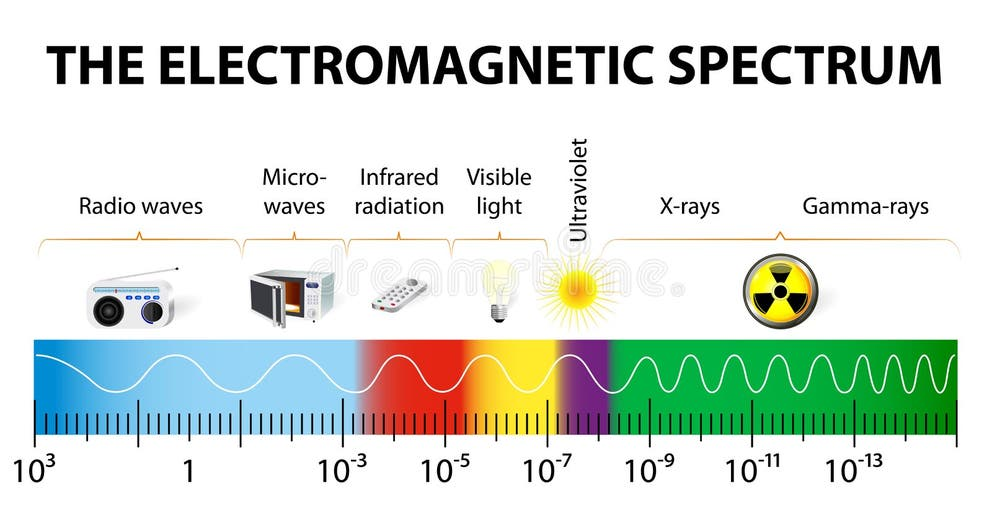
\includegraphics[width=\columnwidth]{Figures/radiation.jpg}}\phantomsection\label{radiation}

\caption{Schematic representation showing the radiation spectrum with decreasing wavelength (in meters) from left to right, radio waves have wavelength of kilometers (that is what it needs to be in our houses from a transmitter tower), microwaves of about 5 cm (easy guess as the size of the box itself is about 15 cm or so) while the visible radiation is 400-800 nano meter.}
\end{figure}

Then we can refer to the figure by saying is shown in the Figure \DUrole{ref}{radiation}

\subsection{Citing People%
  \label{citing-people}%
}


\DUrole{cite}{schmidt2018} \DUrole{cite}{weigert2020} \DUrole{cite}{Beucher2018} \DUrole{cite}{Ronn2015} \DUrole{cite}{Wolny2020} \DUrole{cite}{eschweiler2018}
\bibliographystyle{alphaurl}
\bibliography{vkc}

\end{document}
